\documentclass[12pt,a4paper]{article}
\usepackage[utf8]{inputenc}
\usepackage[english]{babel}
\usepackage{amsmath}
\usepackage{amsfonts}
\usepackage{amssymb}
\usepackage{graphicx}
\graphicspath{ {./graphics/} }

\usepackage[top=1.5in, bottom=1in, left=1in, right=1in]{geometry}


\usepackage{float}

\usepackage{tikz}
\usetikzlibrary{arrows,automata, positioning,calc,shapes.geometric}

% header
\usepackage{fancyhdr}
\pagestyle{fancyplain}
\fancyhf{}
\lhead{ \fancyplain{}{Lukas Schwartz \& Aitor Miguel } }
\rhead{ \fancyplain{}{AI1 - 1. Semester MSc Robot Systems} }
\cfoot{ \fancyplain{}{\thepage} }

% make tables prettyer
\def\arraystretch{1.3}

\usepackage{todonotes}

\begin{document}

\begin{titlepage}
	\centering
%	\includegraphics[width=0.15\textwidth]{example-image-1x1}\par\vspace{1cm}
	\vfill
	{\scshape\LARGE University of Southern Denmark\par}
	\vspace{1cm}
	{\scshape\Large AI1 Project \#1\par}
	{\scshape\large 1. Semester MSc Robot Systems\par}
	\vspace{1.5cm}
	{\huge\bfseries Sokoban Solver\par}
	\vspace{2cm}
	{\Large\itshape Aitor Miguel Blanco \& Lukas Chr. M. W. Schwartz \\ Group \#1 \par}
	\vfill
	supervised by\par
	xyz

	\vspace{2cm}

% Bottom of the page
	{\large 3$^{rd}$ December 2015 \par}
\end{titlepage}

\pagebreak

\tableofcontents

\pagebreak

\listoffigures

\listoftables

\pagebreak

\section{Introduction}

In this project, the problem of solving automatically the sokoban game has been faced.
To do this, the project has been divided in two different parts, being studied separately.
These are finding the shortest solution given a sokoban map and the hardware implementation of a robot able to execute the generated path.

The system loads a map and finds a solution offline with a solver. 
The output of this program is a path that the robot should follow. 
This path is loaded onto the robot, which is prepared to execute it on the sokoban map.

The robot designed is made using different LEGO and LEGO Mindstorms parts and an NXT as controller.
And the solver is programmed using C++.

%The solver is based in the A* algorithm and implemented in C++.

\pagebreak
\section{Physical Design}
To solve the sokoban problem a robot capable of performing simple tasks concerned with moving the can and itself around the game map are needed.
The behaviours the robot should be able to perform define how the robot should be formed in order to accomplish its task of solving the sokoban problem.

\subsection{System Behaviours}
The robot was decided to be build upon being able to execute simple behaviours.
The execution of the behaviours would then be controlled from the \textit{Brain},
this is illustrated in figure \ref{fig:behaviourSystem}.

% brain/behaviour diagram
\begin{figure}[H]
\center
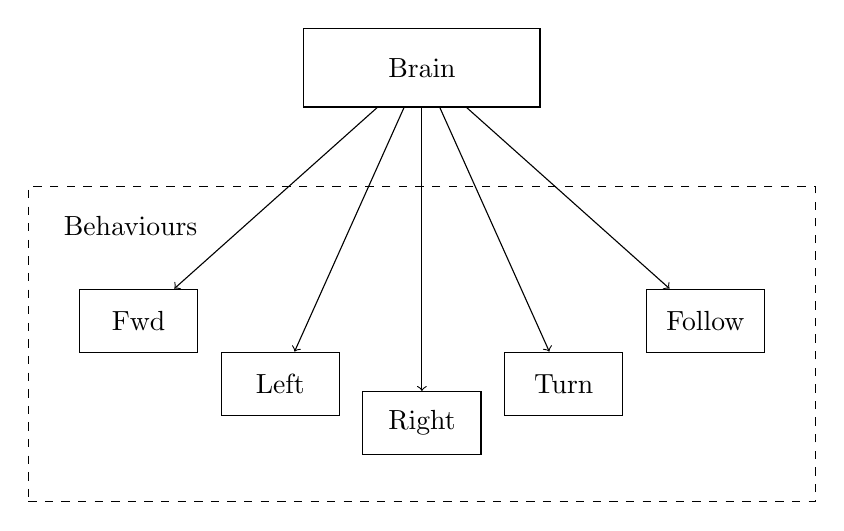
\begin{tikzpicture}[node distance=1cm]
%  behaviour box
\node[rectangle,draw,minimum width=10cm, minimum height=4cm, dashed, name=behaviour_box]  at (0,0) {};
\node[name=behaviour] at (-3.7,1.5) {Behaviours};

% Brain node 
\node[rectangle,draw,minimum width=3cm, minimum height=1cm, name=brain, above=of behaviour_box] {Brain};

% behaviours
\node[rectangle,draw,minimum width=1.5cm, minimum height=0.8cm, name=fwd] at (-3.6,0.3) {Fwd};
\node[rectangle,draw,minimum width=1.5cm, minimum height=0.8cm, name=left] at (-1.8,-0.5) {Left};
\node[rectangle,draw,minimum width=1.5cm, minimum height=0.8cm, name=right] at (0,-1.) {Right};
\node[rectangle,draw,minimum width=1.5cm, minimum height=0.8cm, name=turn] at (1.8,-0.5) {Turn};
\node[rectangle,draw,minimum width=1.5cm, minimum height=0.8cm, name=follow] at (3.6,0.3) {Follow};

% arrows inside 
\draw[->] (brain) -- (fwd) ;
\draw[->] (brain) -- (left) ;
\draw[->] (brain) -- (right) ;
\draw[->] (brain) -- (follow) ;
\draw[->] (brain) -- (turn) ;
\end{tikzpicture}
\caption{Overview of the systems behaviours.}
\label{fig:behaviourSystem}
\end{figure}

Here the central unit, the \textit{Brain} is responsible for finding the solution to the sokoban problem by invoking the five behaviours.
The \textit{Brain} is hence a combination of both the computer processing the map offline and the Lego-robot online when using the offline generated data to solve the puzzle.

The behaviours are defined in table \ref{tab:behaviourExplained} and based on dividing the behaviours into simple tasks which are easy to program.

\begin{table}[H]
\center
\begin{tabular}{c|l}
Behaviour & Description \\ \hline
Fwd & Makes the robot go straight ahead in the next intersection. \\
Left / Right & The robot turns left/right in the next intersection. \\
Turn & Turns the robot 180 degrees around in the next intersection. \\
Follow & Makes the robot follow the line till next intersection.
\end{tabular}
\caption{Behaviour table.}
\label{tab:behaviourExplained}
\end{table}

\todo[inline]{what about a separate push behaviour?}

With these five behaviours the robot should then be able to navigate around the map and when a tomato can is encountered, push it to its destination.
\subsection{Physical Structure}
The structure of the robot should allow the movement of the robot across the map. 
That means, the robot should have at least two motors to move in the plane of the circuit and a minimum of two light sensors to check its position referred to the black lines of the map and check when the robot has arrived to a crossroad.

\subsubsection{Motor configuration and control}
The chosen motor configuration consist in the use of two motors that move two parallel wheels. 
This allows the robot to change the direction of the movement setting a different motor speed on each motor.

To follow the line, the robot should be able to turn, what means that the motors should be set to different speeds.
These speeds are chosen with a P controller.
This controller slows down the speed of one or another wheel in function of the perpendicular displacement of the sensors 
over the line. 


\subsubsection{Sensor configuration}

Three light sensors are used as seen in figure \ref{fig:robotscheme}. 
Two of these sensors are used in the line following control and are placed in the front of the robot.
The distance between them is of 40mm, which is bigger than te line width.
This gives to the controller a big actuation rank, as the distance between the sensors is bigger than the width of the line.

In the position control, the value of the sensors are compared and the robot is controlled having in mind that the value of the sensors should be the same when the robot is centred above the line.
When the value of both sensors are low, the robot is facing a crossroad.


About the third sensor, it is placed in the back of the robot, just before the wheels.
It is used to detect the lines of the crossroads when going back and turning.

This sensor is placed the closest possible to the wheel's axis, and far enough to the robot center so it is not affected
for the followed line.

About the light levels in the room, it has been tested and proved that the sensors are highly sensitive to changes in 
the ambient light levels, specially under sunlight exposure. 

The first solution chosen to solve this problem has been use a shield around the three sensors, so the ambient light 
doesn't affect the measures.
This has shown a good result working in the lab, and under sunlight in cloudy days, but was unable to work in sunny days,
as the sensors were still afected for the sunlight intensity.
To minimize the effect of the sun, a second shield has been placed covering the robot base, so the sensors are allways in
shadows.
This system has shown to be robust under all conditions.



\subsubsection{Tool configuration}

To be able to push and guide the can across the map, the robot should have a proper tool that allows this task. 
The proposed design consist of two bars placed making an angle that allows the guide of the bottle when driving straight forward, as is shown in figure \ref{fig:robotscheme}.
This configuration allows catching the can even when its position is displaced, making the robot's job more easy.

Considering the rules of the game then the can is not permitted to be pushed left or right and because of that, no special design enabling this are required.


The final build of the robot is seen in figure \ref{fig:robotImage}.

\begin{figure}[H]
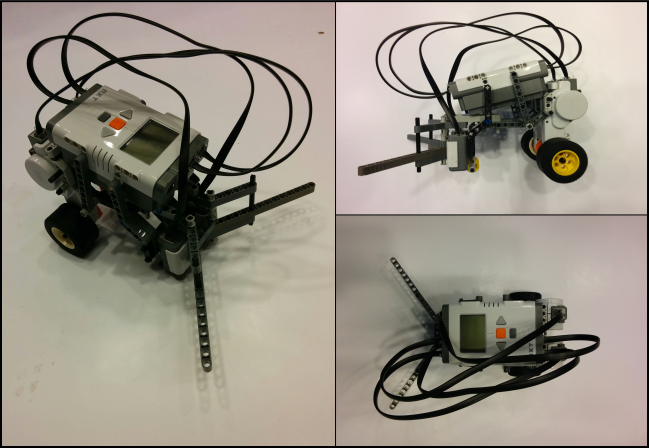
\includegraphics[width=10cm]{Fig1.png}
\centering
\caption{Images of the built robot.}
\label{fig:robotImage}
\end{figure}



\subsection{Tests of the Robot Behaviours}
In order to test the functionality of the behaviours implemented each can be tested individually.
The position controller used in the line following algorithm can be tested by letting the robot drive along a line and record the error of the line sensors.
The smaller it is able to hold the error, the better it is.
Furthermore the line following can be tested with and without the tomato can to check the response when the robot has a load.

To test the turning behaviours the robot can be told to drive in a square and if it is able to maintain the same square, the turning function works.

\todo[inline]{turning both ways? dropping a can after a push?}

\pagebreak
\section{Software}
In order to control and stabilize the segway a the communication with the accelerometer/gyroscope must be established.
This must data received must then be processed in order to control the motors according to the segways position.



\begin{figure}[H]
\centering

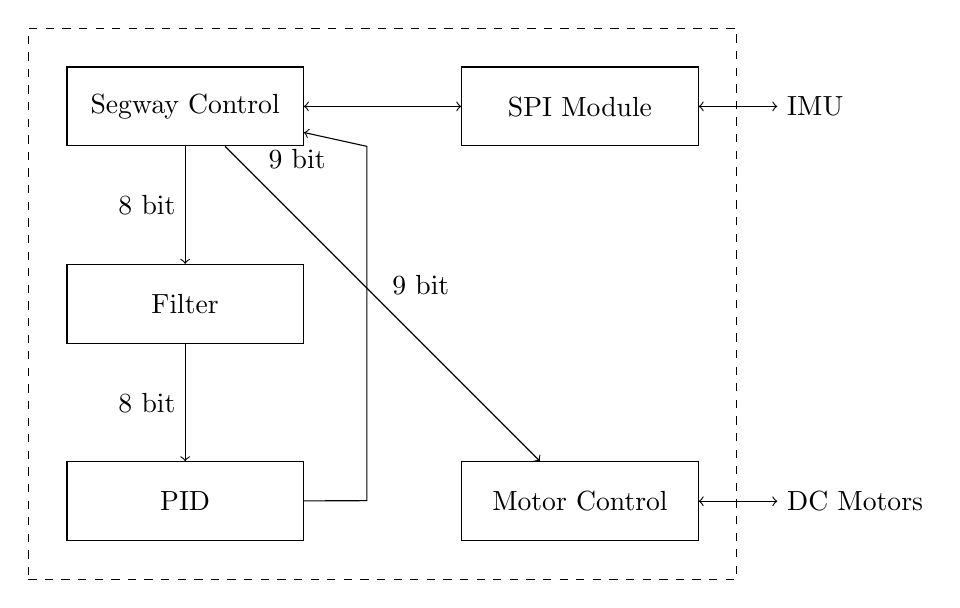
\begin{tikzpicture}[node distance=1cm]
% FPGA border
\node[rectangle,draw,minimum width=9cm, minimum height=7cm, dashed, name=FPGA]  {};

% used to align the insides of FPGA
\node[rectangle,minimum width=5cm, minimum height=5cm, name=FPGAaligne] {};

% components of FPGA
\node[rectangle,draw,minimum width=3cm, minimum height=1cm, name=pid] at (FPGAaligne.-135) {PID};
\node[rectangle,draw,minimum width=3cm, minimum height=1cm, name=communiction] at (FPGAaligne.45) {SPI Module};
\node[rectangle,draw,minimum width=3cm, minimum height=1cm, name=mc] at (FPGAaligne.-45) {Motor Control};
\node[rectangle,draw,minimum width=3cm, minimum height=1cm, name=filter] at (FPGAaligne.180) {Filter};
\node[rectangle,draw,minimum width=3cm, minimum height=1cm, name=segway] at (FPGAaligne.135) {Segway Control};

% nodes outside FPGA
%\node [left=of utos,name=pc] {PC};
\node [right=of communiction,name=spi] {IMU};
%\node [left=of color,name=rgb] {RGB(2:0)};
\node [right=of mc,name=motor] {DC Motors};

% arrows inside FPGA
\draw[<->] (segway) -- node[] {} (communiction) ;
\draw[->] (segway) -- node[left] {8 bit} (filter) ;
\draw[->] (filter) --  node[left] {8 bit} (pid) ;
\draw[->] (segway) -- node[above right] {9 bit} (mc) ;
\draw[->] (pid) --(-0.2,-2.5)--(-0.2,2)-- node[below left] {9 bit} (segway) ;
 
% arrows connected to the outside of FPGA
\draw[<->] (spi) -- node[] {} (communiction) ;
\draw[<->] (mc) -- node[] {} (motor) ;
%\draw[->] (adc) to[out=180, in=0] node[] {} (ad) ;
%\draw[->] (color) to[out=180, in=0] node[] {} (rgb) ;
%\draw[->] (mc) to[out=0, in=180] node[] {} (servo) ;
\end{tikzpicture}

\caption{Block design of the FPGA.}
\label{fig:fpga_sof_design}
\end{figure}


The designed system is comprised by the modules seen in figure \ref{fig:fpga_sof_design}.
Here the \textit{Segway Control} block is the main part of the system, used to combine the different components into one.
The \textit{SPI Module} takes care of the communication with the accelerometer and gyroscope by sending data to such when asked for by the \textit{Segway Control} module.

Data from such is then send to the \textit{Filter} to predict an angle.
From here the angle is passed to the \textit{PID} in order to generate a duty cycle which is then passed back to the main module, the \textit{Segway Control}.
The \textit{Segway Control} hence also takes care to set the right ports on the H-bridges, through the \textit{Motor Control} unit, depending on the speed and direction bit generated by the \textit{PID}.
The five components are explained further throughout this section.





\end{document}